\section{Technology Assessment}
\label{sec:technology}



Introduce in (sufficient) depth the key concepts and architecture of the chosen software technology. As part if this, you may consider using a running example to introduce the technology.

This part and other parts of the report probably needs to refer to
figures. Figure~\ref{fig:framework} from \cite{brown:96} just
illustrates how figure can be included in the report.

\begin{figure}[thb]
	\centering
	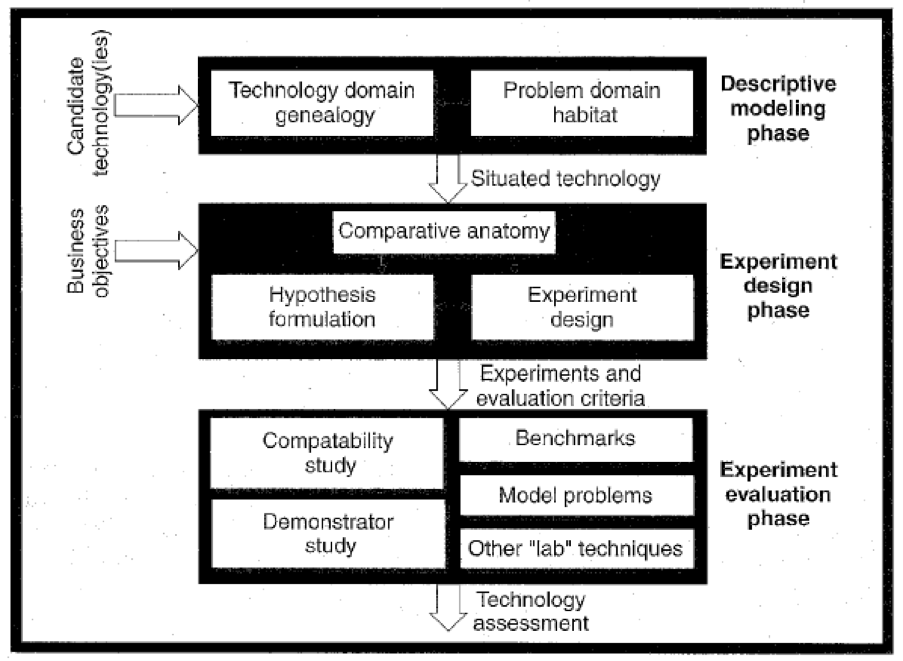
\includegraphics[scale=0.5]{figs/framework.png}
	\caption{Software technology evaluation framework.}
	\label{fig:framework}
\end{figure}

\subsection{Descriptive Modeling}

write where the technology comes from, its history, its context and what problem it solves.
Consider drawing a graph like in \cite{brown:96}.


Kotlin, developed by JetBrains (the Czech software company behind IntelliJ IDEA), is named after Kotlin Island in the Gulf of Finland, near St. Petersburg. JetBrains introduced Kotlin in 2011 as a modern language addressing limitations encountered with Java. The first stable release (Kotlin 1.0) arrived in 2016 and gained traction among Android developers quickly. In 2017, Google endorsed Kotlin as an official language for Android development, a significant boost in adoption. In 2020, JetBrains and Google launched the Kotlin Foundation, solidifying its role in JVM and Android development. Kotlin’s ongoing development focuses on multi-platform capabilities, broadening its use beyond JVM and Android to include web, iOS, and server applications. Kotlin is a statically typed language that compiles to Java bytecode, running on the Java Virtual Machine (JVM), which allows compatibility with Java libraries and frameworks. Designed for safety, conciseness, and interoperability with Java, Kotlin is particularly valuable in three contexts:

\begin{itemize}
    \item \textbf{Android Development}: Kotlin’s concise syntax and enhanced safety features make it a preferred choice in Android development.
    \item \textbf{Server-Side Development}: Kotlin’s seamless integration with JVM-based frameworks like Spring Boot facilitates its use in server applications.
    \item \textbf{Multi-Platform Development}: Kotlin Multiplatform and Kotlin/Native enable shared codebases across platforms, including mobile, web, and desktop applications.
\end{itemize}



\begin{tikzpicture}[node distance=2cm]

\hspace*{-1.5cm}  % Shifts everything 1.5 cm to the left

% Define block styles
\tikzstyle{block} = [rectangle, rounded corners, minimum width=3cm, minimum height=1cm, text centered, draw=black, fill=blue!20]
\tikzstyle{problem} = [rectangle, rounded corners, minimum width=3cm, minimum height=1cm, text centered, draw=black, fill=red!20]
\tikzstyle{context} = [ellipse, minimum width=4cm, minimum height=1cm, text centered, draw=black, fill=yellow!20]
\tikzstyle{arrow} = [thick,->,>=stealth]
\tikzstyle{usecase} = [rectangle, rounded corners, minimum width=3.5cm, minimum height=1cm, text centered, draw=black, fill=green!20]

% Nodes
\node (problem1) [problem] {Problem 1: Verbose Code};
\node (problem2) [problem, below of=problem1] {Problem 2: Null Safety};
\node (problem3) [problem, below of=problem2] {Problem 3: Complex Asynchronous Code};
\node (context) [context, right of=problem2, xshift=4cm] {Context: Java Development};
\node (kotlin) [block, below of=context, yshift=-1cm, minimum width=4cm, minimum height=1.25cm, font=\large] {Kotlin};

% Spread out the blue boxes
\node (feature1) [block, below of=kotlin, xshift=-4cm] {Concise Syntax};
\node (feature2) [block, below of=kotlin] {Null Safety};
\node (feature3) [block, below of=kotlin, xshift=4cm] {Coroutines};

% Spread out the benefits
\node (benefit1) [block, below of=feature1] {Reduced Boilerplate};
\node (benefit2) [block, below of=feature2] {Enhanced Safety};
\node (benefit3) [block, below of=feature3] {Improved Concurrency};

% Use cases (stacked vertically)
\node (usecase1) [usecase, above of=context, xshift=6cm] {Android Development};
\node (usecase2) [usecase, below of=usecase1] {Server-Side Development};
\node (usecase3) [usecase, below of=usecase2] {Multi-Platform Development};

% Arrows
\draw [arrow] (problem1) -- (context);
\draw [arrow] (problem2) -- (context);
\draw [arrow] (problem3) -- (context);
\draw [arrow] (context) -- (kotlin);
\draw [arrow] (kotlin) -- (feature1);
\draw [arrow] (feature1) -- (benefit1);
\draw [arrow] (kotlin) -- (feature2);
\draw [arrow] (feature2) -- (benefit2);
\draw [arrow] (kotlin) -- (feature3);
\draw [arrow] (feature3) -- (benefit3);

% Arrows from use cases to context (yellow oval)
\draw [arrow] (usecase1) -- (context);
\draw [arrow] (usecase2) -- (context);
\draw [arrow] (usecase3) -- (context);

\end{tikzpicture}

\vspace{1cm}

Kotlin is addressing some of Java's limitations. Kotlin as a programming language has many strengths:
\\
\textbf{Conciseness and Readability}: Kotlin’s streamlined syntax reduces repetitive code, improving readability and maintainability. This conciseness also minimizes potential sources of error and makes the codebase easier to work with.
\\
\textbf{Null Safety}: Kotlin’s type system helps prevent NullPointerExceptions by distinguishing between nullable and non-nullable types. This feature significantly reduces bugs related to null handling, a frequent issue in Java.
\\
\textbf{Asynchronous Programming with Coroutines}: Kotlin’s coroutines offer a simplified approach to asynchronous programming, enabling more efficient, non-blocking code execution ideal for network requests or tasks involving resource waits.
\\\
\textbf{Interoperability with Java}: Kotlin’s full compatibility with Java allows teams to gradually integrate Kotlin into existing Java applications. This flexibility is advantageous for modernization efforts without requiring a complete code rewrite.
\\
\textbf{Multi-Platform Support}: Kotlin’s multiplatform capabilities allow for shared business logic across platforms, reducing code duplication and streamlining development for applications targeting Android, iOS, web, and server environments.
\\
\textbf{Functional Programming Features}: Kotlin includes extension functions, higher-order functions, and lambdas, allowing more expressive, modular code. These features support functional programming, further enhancing code flexibility and promoting cleaner architecture.
\\
\textbf{Data Classes}: Kotlin’s data classes simplify the creation of classes primarily used for holding data by automatically generating common methods like \texttt{equals()}, \texttt{hashCode()}, and \texttt{toString()}, streamlining data handling.


\subsection{Experiments: Is Kotlin bettter suited for the PollApp than Java? }

Write you hypotheses about what benefits the technology bring and how you can support or reject them via experiments.

In this section, we present a series of hypotheses regarding the potential benefits of using Kotlin over Java, along with experimental designs that could help validate or refute these assumptions. We are comparing Kotlin and Java code to see the differences between the languages. The concepts discussed in the examples will also apply to our PollApp.

\\
\\
\textbf{Hypothesis 1: Using Kotlin will provide better development speed and code conciseness than Java.} Kotlin’s syntax is designed to be more compact and expressive, which should reduce the time required to implement core functionalities such as user, poll, and vote management. To test this hypothesis, we can compare the time it takes to implement key features in both Kotlin and Java, while also measuring the number of lines of code required to achieve the same outcomes. We come up with a simple example for a class we call person, and compare the lines of code (LOC) to the same class implemented in Java. Our PollApp uses many classes, so a simple class structure is very beneficial:

\textbf{Experiment Example}:
\begin{itemize}
    \item \textbf{Kotlin} (Data class):
    \begin{verbatim}
    data class Person(val name: String, val age: Int)
    \end{verbatim}
    
    \item \textbf{Java} (Full class):
    \begin{verbatim}
    public class Person {
        private String name;
        private int age;

        public Person(String name, int age) {
            this.name = name;
            this.age = age;
        }

        public String getName() { return name; }
        public int getAge() { return age; }
        @Override public String toString() { 
   	        return "Person{name='" + name + "', age=" + age + '}'; 
        }
    }
    \end{verbatim}
\end{itemize}

\textbf{Evaluation}: We see from the examples that Java are using significant more lines of code than Kotlin to achieve the same functionality.  Kotlin's \texttt{data class} reduces the need for boilerplate code (like getters, setters, and \texttt{toString()}), making the code more concise and error-resistant. Java’s verbose approach introduces potential for mistakes and increases code length.
\\
\\
\textbf{Conclusion}: The hypothesis holds. 
\\
\\
\textbf{Hypothesis 2: Using Kotlin will result in fewer runtime exceptions related to null pointer errors compared to Java}:  Null pointer errors can happen in situations where entities like users, polls, or votes do not exist even though they are expected to. These kinds of errors are common in Java, where null checks must be manually implemented. To evaluate this, we could introduce null values in critical parts of the business logic (e.g., missing users or votes) and compare the frequency of runtime exceptions between Kotlin and Java. By observing how each language handles missing data, we can assess Kotlin’s ability to enhance application stability. We will not test this in our case, but we will provide a small example that highlights why Java are more prone to null pointer errors than Kotlin.

\textbf{Experiment Example}:
\begin{itemize}
    \item \textbf{Kotlin} (Null safety):
    \begin{verbatim}
    fun greet(name: String?) {
        println("Hello, ${name ?: "Guest"}!")
    }
    greet(null)  // Output: Hello, Guest!
    \end{verbatim}
    
    \item \textbf{Java} (Manual null check):
    \begin{verbatim}
    public void greet(String name) {
        if (name == null) {
            name = "Guest";
        }
        System.out.println("Hello, " + name);
    }
    greet(null);  // Output: Hello, Guest!
    \end{verbatim}
\end{itemize}

\textbf{Evaluation}: From the examples we see that Kotlin is designed so that it does not need to handle null checks manually. Kotlin’s \texttt{null} safety ensures that nullability is explicitly handled using \texttt{?} and \texttt{?:}, reducing runtime errors. Java’s manual null checks are error-prone and can be easily missed, leading to potential \texttt{NullPointerException} risks.
\\
\\
\textbf{Conclusion}: The hypothesis holds. 
\\
\\
\textbf{Hypothesis 3: Kotlin's coroutines offer a more efficient and readable approach to handling asynchronous tasks compared to Java}: Kotlin's coroutines are expected to improve response times and scalability when handling a high volume of voting requests. To test this, we would implement the voting logic using Kotlin coroutines and then simulate high traffic scenarios, comparing the application’s performance with a similar Java implementation using traditional concurrency methods like threads. Key metrics such as response time and memory usage would be tracked to determine which language offers better scalability under load. In our case we choose to have another code example to prove our hypothesis instead. 
\\
\\
\textbf{Experiment Example}:
\begin{itemize}
    \item \textbf{Kotlin} (Coroutines):
    \begin{verbatim}
    import kotlinx.coroutines.*

    suspend fun fetchData() {
        delay(1000)
        println("Data fetched")
    }

    fun main() = runBlocking {
        launch { fetchData() }
    }
    \end{verbatim}
    
    \item \textbf{Java} (Threads):
    \begin{verbatim}
    public class Main {
        public static void fetchData() {
            try {
                Thread.sleep(1000);
                System.out.println("Data fetched");
            } catch (InterruptedException e) {
                e.printStackTrace();
            }
        }

        public static void main(String[] args) {
            Thread thread = new Thread(() -> fetchData());
            thread.start();
        }
    }
    \end{verbatim}
\end{itemize}

\textbf{Conclusion}: Kotlin coroutines simplify asynchronous code, making it more readable and reducing boilerplate. Java’s thread-based approach requires more code and is harder to manage due to explicit thread handling and synchronization.

\\
\\
Finally, we hypothesize that Kotlin Multiplatform could reduce code duplication and improve consistency across platforms by enabling shared code between the backend and a mobile client. To experiment with this, we could develop a prototype that shares core voting functions between the backend and an Android client. By measuring the amount of duplicated code and assessing the maintenance requirements for each platform, we can evaluate the potential benefits of using Kotlin Multiplatform in terms of consistency and ease of maintenance.
\\
\\
The hypothesis regarding Kotlin’s concise syntax posits that Kotlin’s data class feature will allow for more compact and error-resistant code compared to Java's verbose approach. For instance, in Kotlin, a simple data class can be defined in just one line, eliminating the need for boilerplate code such as getters, setters, and a \texttt{toString()} method. Java, on the other hand, requires the full definition of a class with explicit methods for each of these actions, which increases the likelihood of errors and results in more lines of code.
\\
\\
In terms of null safety, Kotlin offers built-in mechanisms that handle nullability explicitly through the use of the \texttt{?} operator and the \texttt{?:} Elvis operator, which reduces the risk of \texttt{NullPointerException} errors that are common in Java when manual null checks are missed. This feature ensures that nullability is addressed in a clear and safe manner, whereas Java requires developers to implement their own null checks, which can be error-prone and overlooked.

Kotlin’s coroutines also promise a more efficient and readable way to handle asynchronous tasks compared to Java’s thread-based model. With coroutines, asynchronous code is written in a sequential manner, avoiding the complexity of managing threads and synchronization. In contrast, Java requires the explicit creation of threads and the management of their execution, which introduces additional boilerplate code and complexity. As such, Kotlin’s coroutines simplify asynchronous programming and improve the overall readability of the code.

Through these experiments, we can assess the various advantages Kotlin offers over Java, particularly in terms of development speed, code safety, asynchronous handling, and cross-platform code sharing.


\maketitle

\section*{Improved Development Speed and Code Conciseness}

\textbf{Hypothesis:} Using Kotlin will reduce development time due to its concise syntax. This is expected to simplify tasks such as user, poll, and vote management.

\textbf{Experiment:} Compare the implementation time for key functionalities (e.g., user creation, poll management, and vote handling) between Kotlin and Java. Measure the lines of code required to implement the same logic in both languages and track developer productivity through task completion rates.

\section*{Enhanced Safety with Null Safety}

\textbf{Hypothesis:} Kotlin’s null safety features will reduce runtime exceptions related to null pointer errors, especially in scenarios where entities (like User, Poll, or Vote) might not exist, which would otherwise cause crashes in Java.

\textbf{Experiment:} Introduce null values in critical parts of the business logic (e.g., missing users or votes) and measure the number of runtime exceptions in both Kotlin and Java. Monitor the resilience of the application in handling missing data.

\section*{Simplified Asynchronous Voting Process}

\textbf{Hypothesis:} Kotlin coroutines will streamline asynchronous handling of voting logic, improving response time and scalability during high voting activity.

\textbf{Experiment:} Implement the voting logic using Kotlin coroutines, then simulate high volumes of voting requests. Compare the application’s response times and memory usage with a similar Java implementation using standard concurrency methods.

\section*{Cross-Platform Code Sharing Potential}

\textbf{Hypothesis:} Kotlin Multiplatform would enable code sharing for the voting logic between a potential mobile client and backend, reducing duplicated logic and ensuring consistency across platforms.

\textbf{Experiment:} Set up a prototype of a shared code module containing core voting functions for both the backend and an Android client. Measure code duplication and maintenance requirements, assessing potential consistency improvements.


\subsection{Experiment Evaluation}

Write about the results of your experiments, either via personal experience reports, quantitative benchmarks, a demostrator case study or a combination of multiple approaches.


For some reports you may have to include a table with experimental
results are other kinds of tables that for instance compares
technologies. Table~\ref{tab:results} gives an example of how to create a table.

\begin{table}[bth]
	\centering
	\begin{tabular}{llrrrrrr}
		Config & Property & States & Edges & Peak & E-Time & C-Time & T-Time
		\\ \hline \hline
		22-2 & A   &    7,944  &   22,419  &  6.6  \%  &  7 ms & 42.9\% &  485.7\% \\
		22-2 & A   &    7,944  &   22,419  &  6.6  \%  &  7 ms & 42.9\% &  471.4\% \\
		30-2 & B   &   14,672  &   41,611  &  4.9  \%  & 14 ms & 42.9\% &  464.3\% \\
		30-2 & C   &   14,672  &   41,611  &  4.9  \%  & 15 ms & 40.0\% &  420.0\% \\ \hline
		10-3 & D   &   24,052  &   98,671  & 19.8  \%  & 35 ms & 31.4\% &  285.7\% \\
		10-3 & E   &   24,052  &   98,671  & 19.8  \%  & 35 ms & 34.3\% &  308.6\% \\
		\hline \hline
	\end{tabular}
	\caption{Selected experimental results on the communication protocol example.}
	\label{tab:results}
\end{table}


\section*{1. Concise Syntax}

\textbf{Hypothesis}: Kotlin's syntax will be more concise and less error-prone compared to Java’s verbose syntax.

\textbf{Experiment Example}:
\begin{itemize}
    \item \textbf{Kotlin} (Data class):
    \begin{verbatim}
    data class Person(val name: String, val age: Int)
    \end{verbatim}
    
    \item \textbf{Java} (Full class):
    \begin{verbatim}
    public class Person {
        private String name;
        private int age;

        public Person(String name, int age) {
            this.name = name;
            this.age = age;
        }

        public String getName() { return name; }
        public int getAge() { return age; }
        @Override public String toString() { return "Person{name='" + name + "', age=" + age + '}'; }
    }
    \end{verbatim}
\end{itemize}

\textbf{Conclusion}: Kotlin's \texttt{data class} reduces the need for boilerplate code (like getters, setters, and \texttt{toString()}), making the code more concise and error-resistant. Java’s verbose approach introduces potential for mistakes and increases code length.

\section*{2. Null Safety}

\textbf{Hypothesis}: Kotlin’s null safety features will reduce runtime errors due to null dereferencing compared to Java’s manual null checks.

\textbf{Experiment Example}:
\begin{itemize}
    \item \textbf{Kotlin} (Null safety):
    \begin{verbatim}
    fun greet(name: String?) {
        println("Hello, ${name ?: "Guest"}!")
    }
    greet(null)  // Output: Hello, Guest!
    \end{verbatim}
    
    \item \textbf{Java} (Manual null check):
    \begin{verbatim}
    public void greet(String name) {
        if (name == null) {
            name = "Guest";
        }
        System.out.println("Hello, " + name);
    }
    greet(null);  // Output: Hello, Guest!
    \end{verbatim}
\end{itemize}

\textbf{Conclusion}: Kotlin’s \texttt{null} safety ensures that nullability is explicitly handled using \texttt{?} and \texttt{?:}, reducing runtime errors. Java’s manual null checks are error-prone and can be easily missed, leading to potential \texttt{NullPointerException} risks.

\section*{3. Coroutines (Asynchronous Programming)}

\textbf{Hypothesis}: Kotlin’s coroutines will provide a more efficient and readable way to handle asynchronous tasks than Java’s traditional threading model.

\textbf{Experiment Example}:
\begin{itemize}
    \item \textbf{Kotlin} (Coroutines):
    \begin{verbatim}
    import kotlinx.coroutines.*

    suspend fun fetchData() {
        delay(1000)
        println("Data fetched")
    }

    fun main() = runBlocking {
        launch { fetchData() }
    }
    \end{verbatim}
    
    \item \textbf{Java} (Threads):
    \begin{verbatim}
    public class Main {
        public static void fetchData() {
            try {
                Thread.sleep(1000);
                System.out.println("Data fetched");
            } catch (InterruptedException e) {
                e.printStackTrace();
            }
        }

        public static void main(String[] args) {
            Thread thread = new Thread(() -> fetchData());
            thread.start();
        }
    }
    \end{verbatim}
\end{itemize}

\textbf{Conclusion}: Kotlin coroutines simplify asynchronous code, making it more readable and reducing boilerplate. Java’s thread-based approach requires more code and is harder to manage due to explicit thread handling and synchronization.

